\section{A motivating example: parkinson's disease}
\label{intro-complete_ex}

Perhaps the best way to discuss the modeling challenges of meta-regression is by an example from the GBD 2010 study.  The GBD 2010 study provides estimates of the disability adjusted life-year (DALYs), a measurement of disease burden.  DALYs include measurements of morbidity and mortality which require disease prevalence or incidence and duration.

Parkinson's disease is a neurodegenerative disorder.  Motor dysfunction, such as tremor, rigidity or akinesia, are symptoms in the early stages of the disease.  After ______, most patients also develop non-motor symptoms, such as cognitive decline, dementia, autonomic failure and disordered sleep-wake regulation.  There is no cure and no known treatments to slow the progression of the disease.  However, motor symptoms and disability may be improved with symptomatic therapy.

Systematic review for Parkinson's disease yielded 660 prevalence, 99 incidence, 1638 cause-specific mortality rate and 13 standardized mortality ratio data points that met the inclusion criteria.  Looking at the data in Figure \ref{fig:intro-parkinsons fit},


Only 36 countries from 12 regions are represented from the systematic review.  The GBD 2010 study predicts country-year-age-sex for all countries, even those without data.  Thus out-of-sample predictions are key.  Covariate modeling, as discussed in Chapters \ref{theory-covariate_modeling} and \ref{applications-efx_country_level} provide a solution to this problem of missing data.


need for confrontation
heterogeneous data

spline
heterogeneous data and overlapping age groups \ref{applications-age_groups} \ref{theory-age_group_model-overlapping_data}
study level fixed effects (diagnostic criteria) \ref{applications-efx_study_level} \ref{theory-covariate_modeling}
country level fixed effects (representative) \ref{applications-efx_country_level} \ref{theory-covariate_modeling}
random effects \ref{applications-rfx} \ref{theory-covariate_modeling}
csmr v pf \ref{applicatoins-csmr} \ref{theory-csmr}

x_cv_ascertainment
x_cv_diagnostic_criteria
x_cv_representative
x_ihme_fao_stimulants_kcal_26oct11
x_smoking_prev

complete discussion of all p, i and pf data points

chronic neurodegenerative disorder
are effective symptomatic therapies
no treatment has yet been identified that would significantly slow its natural progression
motor dysfunction in early stages
non-motor symptoms: dementia, sleep-wake cycle dysregulation and autonomic failure

Symptomatic therapy with dopamine replacement strategies is associated with marked improvement of motor symptoms and disability but has not been shown to significantly alter
the progression of the underlying neuronal degeneration of illness

After prolonged disease duration of 10 or more years a majority of patients will
also have developed a plethora of non-motor symptoms for which there are currently no effective treatments. These include cognitive decline, dementia and psychosis, autonomic failure, sleep-wake-cycle dysregulation as well as depression, pain and sensory symptoms

progression of tremor, rigidity or akinesia
postural instability, freezing of gait, dysphagia and dysarthria
cognitive decline and dementia, autonomic failure, disordered sleep-wake regulation as
well as sensory symptoms and signs

multisystem neuronal degeneration of PD

aggressive progression of motor dysfunction in early PD

neurodegenerative movement disorder related to progressive loss of cholinergic neurons

cognitive decline, dementia,

\cite{poewe_natural_2006}

age of onset had influence over course of disease

    \begin{figure}[h]
        \begin{center}
            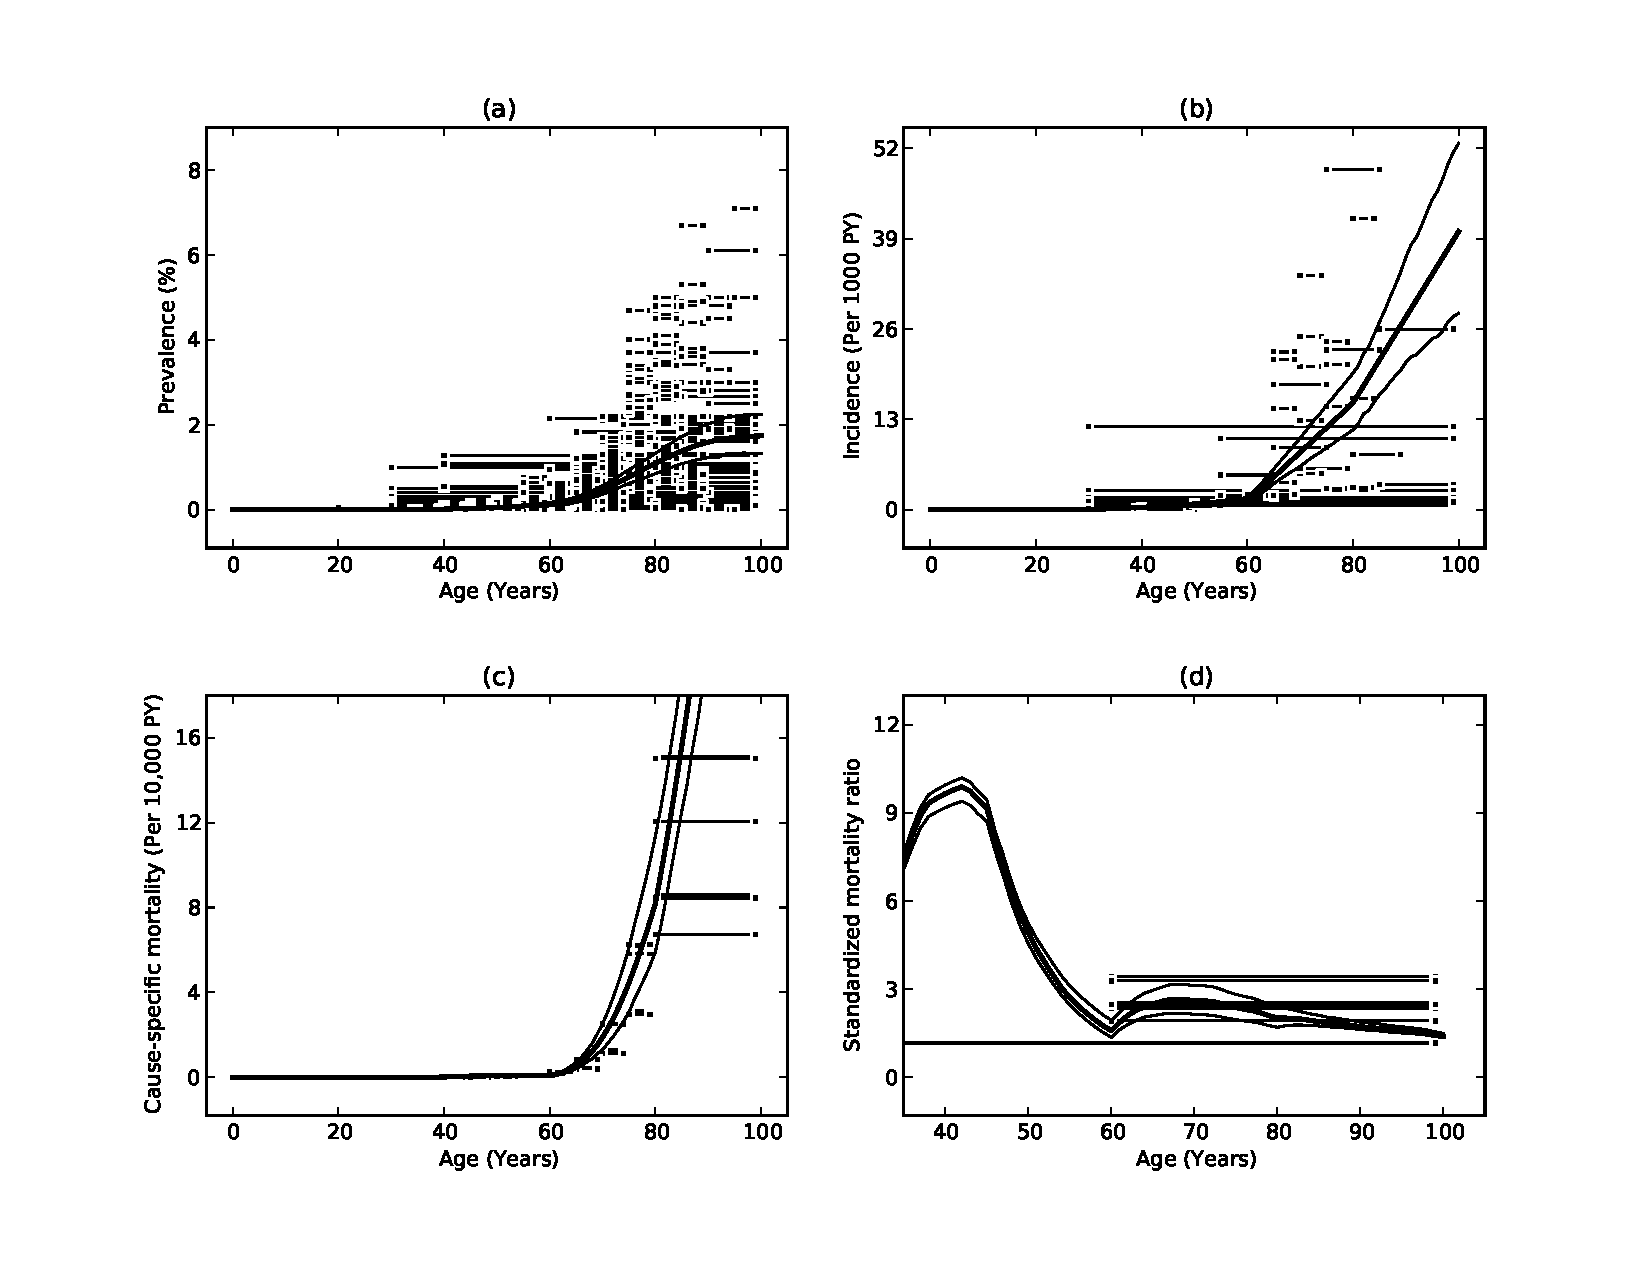
\includegraphics[width=\textwidth]{parkinsons-best.pdf}
            \caption{Estimates of prevalence (panel (a)), incidence (panel (b)), cause-specific mortality (panel (c)) and the standardized mortality ratio of Parkinson's disease in Western European females in 2005.}
            \label{fig:intro-parkinsons fit}
        \end{center}
    \end{figure} 